\documentclass{beamer}

\usepackage{amsmath}
\usepackage{amssymb}
\usepackage{mathtools}
\usepackage{amstext}
\usepackage{amsthm}
\usepackage{fancyhdr}
\usepackage{siunitx}
\usepackage{physics}

\usepackage{hyperref}


\usepackage{graphicx}
\usepackage{float}
\graphicspath{{figures/}} %Setting the graphicspath
\usepackage{float}
\usepackage{caption}
\usepackage{subcaption}

% To work with inkfigures
\usepackage{import}
\usepackage{pdfpages}
\usepackage{transparent}
\usepackage{xcolor}

\newcommand{\angstrom}{\textup{\AA}}
\numberwithin{equation}{section}
\renewcommand\thesubsection{\alph{subsection})}
\renewcommand\thesubsubsection{\Roman{subsubsection}}
\newcommand{\s}{\hspace{0.1cm}}

%\usetheme{AnnArbor}
%\usetheme{Antibes}
%\usetheme{Bergen}
%\usetheme{Berkeley}
%\usetheme{Berlin}
%\usetheme{Boadilla}
%\usetheme{boxes}
%\usetheme{CambridgeUS}
%\usetheme{Copenhagen}
%\usetheme{Darmstadt}
%\usetheme{default}
%\usetheme{Frankfurt}
%\usetheme{Goettingen}
%\usetheme{Hannover}
%\usetheme{Ilmenau}
%\usetheme{JuanLesPins}
%\usetheme{Luebeck}
\usetheme{Madrid}
%\usetheme{Malmoe}
%\usetheme{Marburg}
%\usetheme{Montpellier}
%\usetheme{PaloAlto}
%\usetheme{Pittsburgh}
%\usetheme{Rochester}
%\usetheme{Singapore}
%\usetheme{Szeged}
%\usetheme{Warsaw}

% Astronomy
\DeclareSIUnit\parsec{pc}
\DeclareSIUnit\lightyear{ly}


\institute[] % (optional, but mostly needed)
{
		Département de Physique\\
		Université de Montréal
}
\title{Mesure de $H_0$}
\subtitle{Détermination du potentiel de Fermat de la lentille RXJ1131-1231}

\author{Alexandre Adam, \\ 
        Charles Wilson}

\date{PHY6669 -- Cosmologie}

\AtBeginSubsection[]
{
  \begin{frame}<beamer>{Résumé}
	\tableofcontents[currentsection,currentsubsection]
  \end{frame}
}

\usepackage[authoryear]{natbib}
\bibliographystyle{abbrvnat}
\captionsetup{labelformat=empty,labelsep=none}

\begin{document}

\begin{frame}
	\titlepage
\end{frame}


\begin{frame}{Résumé}
	\tableofcontents
\end{frame}

\section{Contexte}
\subsection{Mesures}

\begin{frame}{Mesures}{Planck (2018) + $\Lambda$CDM}
        \begin{figure}[H]
                \centering
                \includegraphics[width=\textwidth]{TT_power_spectra_Planck2018}
                \caption{Mesure indirecte: $\boxed{100h = 67.36 
                        \pm 0.54\,\, (0.8\%)}$ à $z \gtrsim 1100$
                \footnote{\citet{PlanckCollaboration2018}}}
        \end{figure}
        	
\end{frame}

\begin{frame}{Mesures}{Sh0es (Riess \textit{et al.})}
        \begin{figure}[H]
                \centering
                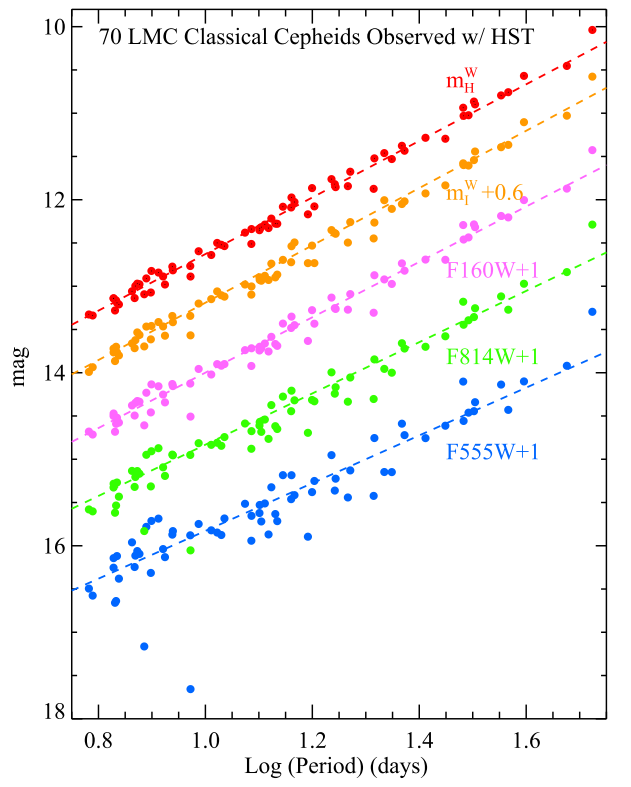
\includegraphics[width=0.4\textwidth]{Sh0es_mesure}
                \caption{Mesure directe: $\boxed{100h = 74.03 \pm 1.42\,\,(1.9\%)}$ à $z\ll 1$
                \footnote{\citet{Riess2019}}}
        \end{figure}
\end{frame}

\begin{frame}{Mesures}{H0LiCOW (Suyu \textit{et al.})}
        \begin{figure}[H]
                \centering
                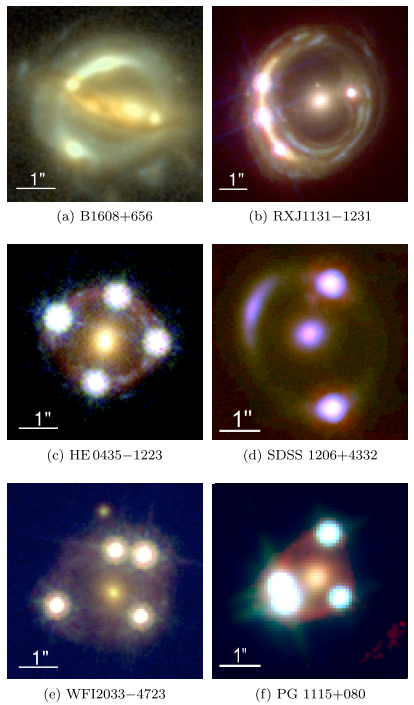
\includegraphics[width=0.25\textwidth]{holicow_lens}
                \caption{Mesure semi-direct: 
                $\boxed{100h = 73.3^{+1.7}_{-1.8}\,\,(2.4\%)}$ avec 
                        $z_\ell \sim 0.5$ et $z_s \lesssim 2$.
                \footnote{\citet{Wong2020}}}
        \end{figure}
\end{frame}

\subsection{Tension}
\begin{frame}{Tension}
        \begin{figure}[H]
                \centering
                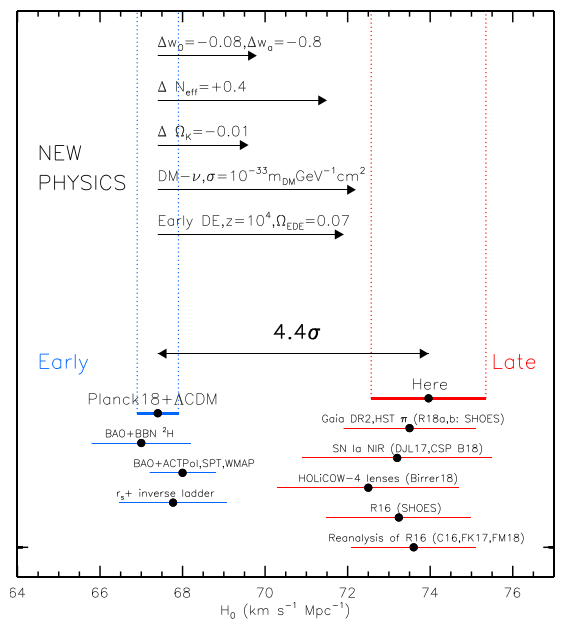
\includegraphics[width=0.4\textwidth]{H0_tension_Sh0es2019}
                \caption{
                        \footnote{\citet{Riess2019}}
                        Les mesures locales sont en conflit avec $H_0$ dérivée du CMB, 
                des oscillations acoustiques baryoniques (BAO) et de la nucléosynthèse 
        di Big Bang (BBN)}
        \end{figure}
         
\end{frame}

\section{RXJ1131-1231}
\begin{frame}
		
\end{frame}

\section{Reconstruction}
\begin{frame}
		
\end{frame}

\begin{frame}[allowframebreaks]{Référence}
        \bibliography{bibliography.bib}
        
\end{frame}

\end{document}

